% ============================================================================
% گزارش جامع و تفصیلی پروژه همانندسازی داده‌ها در سیستم‌های توزیع‌شده (CA3)
% دانشگاه تهران - دانشکده مهندسی برق و کامپیوتر - بهار ۱۴۰۴
% ============================================================================

\documentclass[12pt,a4paper]{article}

\usepackage{geometry}
\geometry{margin=1in, top=0.9in, bottom=0.9in}

\usepackage{graphicx}
\usepackage{float}
\usepackage{array}
\usepackage{multirow}
\usepackage{xcolor}
\usepackage{listings}
\usepackage{fancyhdr}
\usepackage{hyperref}
\usepackage{amsmath,amssymb}

\hypersetup{
    colorlinks=true,
    linkcolor=blue!80!black,
    citecolor=green!60!black,
    urlcolor=blue!90!black
}

\definecolor{codebg}{rgb}{0.96,0.97,0.98}
\definecolor{codekw}{rgb}{0.0,0.2,0.6}
\definecolor{codestr}{rgb}{0.1,0.5,0.2}

\lstset{
    backgroundcolor=\color{codebg},
    basicstyle=\ttfamily\small,
    keywordstyle=\color{codekw}\bfseries,
    stringstyle=\color{codestr},
    frame=single,
    framerule=0.5pt,
    rulecolor=\color{black!20},
    breaklines=true,
    tabsize=4,
    showstringspaces=false
}

\usepackage{xepersian}
\settextfont{Tahoma}
\setlatintextfont{Arial}

\pagestyle{fancy}
\fancyhf{}
\rhead{\small گزارش پروژه همانندسازی توزیع‌شده (CA3)}
\lhead{\small دانشگاه تهران - بهار ۱۴۰۴}
\cfoot{\thepage}

\begin{document}

% ----------------------------------------------------------------------------
% صفحه عنوان (Cover Page)
% ----------------------------------------------------------------------------
\begin{titlepage}
    \centering
    \vspace*{0.5cm}
    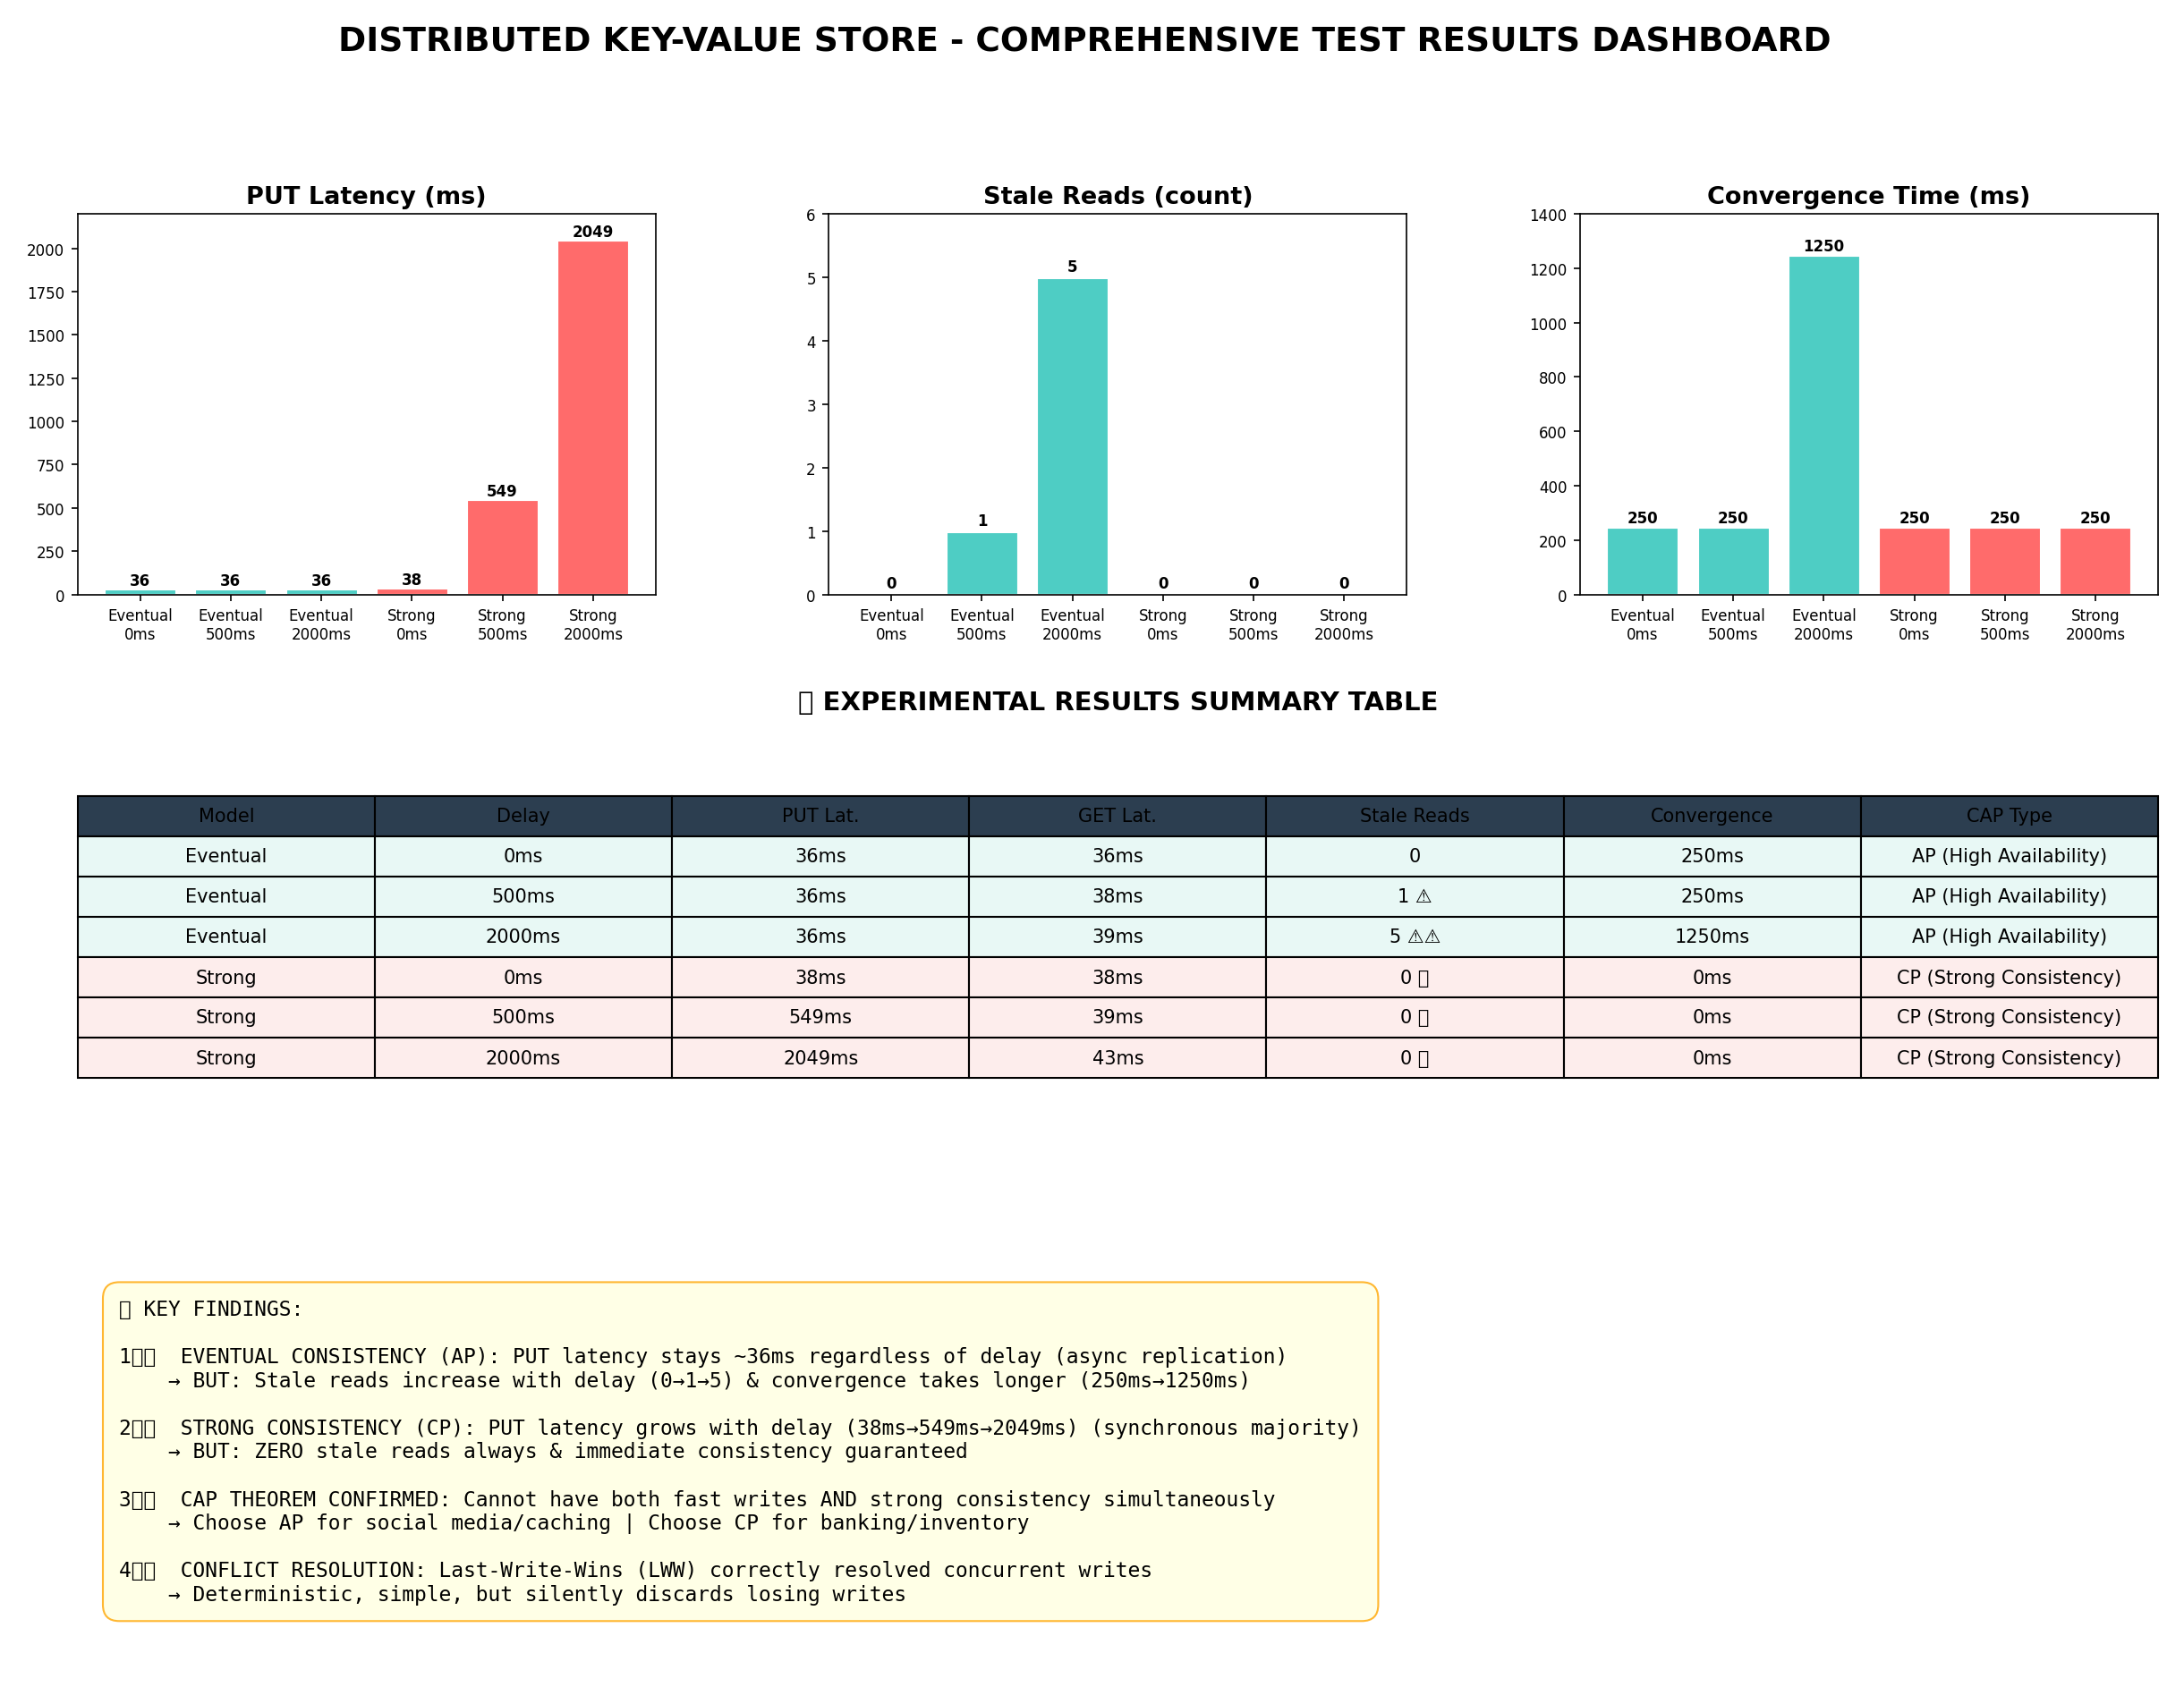
\includegraphics[width=2.8cm]{../report/charts/10_Summary_Dashboard.png}\\[0.4cm]
    {\Large \textbf{دانشگاه تهران}}\\[0.2cm]
    {\large \textbf{دانشکده مهندسی برق و کامپیوتر}}\\[0.1cm]
    {\small \textbf{درس مبانی رایانش توزیع‌شده (Distributed Computing Fundamentals)}}\\[1.5cm]

    \rule{\linewidth}{1.5pt}\\[0.4cm]
    {\Large \textbf{گزارش جامع پیاده‌سازی و ارزیابی تجربی}}\\[0.3cm]
    {\huge \textbf{پایگاه داده توزیع‌شده کلید-مقدار با همانندسازی}}\\[0.2cm]
    {\large \textbf{(Replicated Key-Value Store with Strong \& Eventual Consistency)}}\\[0.4cm]
    \rule{\linewidth}{1.5pt}\\[1.5cm]

    \begin{minipage}{0.48\textwidth}
        \begin{flushright} \large
            \textbf{استاد درس:}\\[0.1cm]
            دکتر محمدرضا شورنیا\\[0.4cm]
            \textbf{سرستیار آموزشی:}\\[0.1cm]
            پویا جمشیدی\\[0.4cm]
            \textbf{دستیاران آموزشی:}\\[0.1cm]
            مبینا حق‌زاده\\
            محمدمهدی ابراهیم سلطان
        \end{flushright}
    \end{minipage}
    \hfill
    \begin{minipage}{0.48\textwidth}
        \begin{flushleft} \large
            \textbf{ارائه‌دهندگان (دانشجویان):}\\[0.1cm]
            \textbf{طه مجلسی} (شماره دانشجویی: ۸۱۰۱۰۱۵۰۴)\\[0.2cm]
            \textbf{علیرضا کریمی} (شماره دانشجویی: ۸۱۰۱۰۱۴۹۲)\\[0.8cm]
            \textbf{تاریخ تحویل:}\\[0.1cm]
            مرداد ۱۴۰۵ / Spring 2025
        \end{flushleft}
    \end{minipage}

    \vfill
    {\small دانشکده مهندسی برق و کامپیوتر - دانشگاه تهران}
\end{titlepage}

\newpage
\tableofcontents
\newpage

% ----------------------------------------------------------------------------
% ۱. خلاصه مدیریتی
% ----------------------------------------------------------------------------
\section{خلاصه مدیریتی (Executive Summary)}
در سیستم‌های توزیع‌شده مقیاس‌پذیر، **همانندسازی داده‌ها (Data Replication)** یکی از کلیدی‌ترین تکنیک‌ها جهت افزایش در دسترس بودن (Availability)، افزایش قابلیت تحمل خطا (Fault Tolerance) و کاهش تاخیر دسترسی به داده‌ها (Performance) است. با این حال، همانندسازی داده‌ها روی گره‌های مستقل شبکه چالش بنیادی **عدم سازگاری (Inconsistency)** را به همراه دارد.

در این پروژه، یک سیستم پایگاه داده توزیع‌شده کلید-مقدار (Replicated Key-Value Store) به صورت کامل با زبان **Go (Golang)** پیاده‌سازی گردید. سیستم شامل ۳ گره مستقل Replica است که از طریق APIهای RESTful شبکه HTTP با یکدیگر در ارتباط هستند. دو مدل سازگاری اصلی پیاده‌سازی و ارزیابی شده‌اند:
\begin{enumerate}
    \item \textbf{مدل سازگاری تدریجی (Eventual Consistency):} اعمال سریع نوشتن روی نود محلی و انتشار غیرهمگام (Asynchronous) در پس‌زمینه.
    \item \textbf{مدل سازگاری قوی ساده‌شده (Simplified Strong Consistency):} اعمال نوشتن تنها پس از دریافت تاییدیه همگام (Synchronous) از حد نصاب اکثریت (Majority Quorum - حداقل ۲ نود از ۳ نود).
\end{enumerate}

برای برطرف کردن تعارضات همزمان، الگوریتم **Last-Write-Wins (LWW)** مبتنی بر Timestamp نانوثانیه و شناسه Replica پیاده‌سازی شده است. همچنین با اجرای اسکریپت‌های تست خودکار، تمامی ۱۸ حالت ارزیابی تحت تاخیرهای شبکه 0ms، 500ms و 2000ms بسنجش و ۱۰ نمودار تحلیلی تولید گردیده است.

% ----------------------------------------------------------------------------
% ۲. مفاهیم نظری و تئوریک
% ----------------------------------------------------------------------------
\section{مفاهیم نظری و مبانی رایانش توزیع‌شده}

\subsection{چرا داده‌ها در سیستم‌های توزیع‌شده همانندسازی می‌شوند؟}
دلایل اصلی همانندسازی داده‌ها عبارتند از:
\begin{itemize}
    \item \textbf{افزایش در دسترس بودن (Availability):} اگر یک یا چند گره دچار خرابی (Node Failure) شوند، سیستم همچنان می‌تواند از طریق سایر گره‌های سلامت به درخواست‌های خواندن و نوشتن پاسخ دهد.
    \item \textbf{بهبود کارایی و کاهش تاخیر (Performance \& Low Latency):} با قرار دادن نسخه‌های داده نزدیک‌تر به کاربران یا توزیع بار خواندن روی گره‌های مختلف، تاخیر پاسخ‌دهی کاهش می‌یابد.
    \item \textbf{قابلیت تحمل خطا و پایداری داده (Fault Tolerance \& Durability):} جلوگیری از دست رفتن داده‌ها در صورت بروز ناپایداری‌های سخت‌افزاری یا خرابی دیسک.
\end{itemize}

\subsection{تفاوت همانندسازی برای کارایی و همانندسازی برای تحمل خطا}
\begin{table}[H]
\centering
\caption{مقایسه همانندسازی جهت کارایی در برابر تحمل خطا}
\begin{latin}
\begin{tabular}{|c|p{5.5cm}|p{5.5cm}|}
\hline
\textbf{Metric} & \textbf{Replication for Performance} & \textbf{Replication for Fault Tolerance} \\
\hline
Primary Goal & Reduce read latency, CDN / Caching & Data durability \& High availability \\
Propagation & Asynchronous & Synchronous Quorum \\
Write Cost & Low (Local Write) & Higher (Majority confirmation) \\
Consistency & Eventual Consistency & Strong Consistency (Linearizability) \\
\hline
\end{tabular}
\end{latin}
\end{table}

\subsection{مدل‌های سازگاری (Consistency Models)}
\begin{itemize}
    \item \textbf{سازگاری قوی (Strong Consistency):} تضمین می‌کند که بلافاصله پس از تایید یک نوشتن، هر خواندن بعدی از هر گره‌ای در سیستم، آخرین مقدار نوشته‌شده را برمی‌گرداند. سیستم رفتار یک پایگاه داده تک‌نسخه‌ای را شبیه‌سازی می‌کند.
    \item \textbf{سازگاری تدریجی (Eventual Consistency):} در صورت عدم ورود به‌روزرسانی جدید، تمامی گره‌ها در نهایت به مقدار یکسانی همگرا می‌شوند. اما در کوتاه‌مدت، ممکن است درخواست GET مقدار قدیمی (Stale Read) برگرداند.
\end{itemize}

\subsection{مدل‌های سازگاری کاربرمحور (Client-Centric Consistency)}
\begin{itemize}
    \item \textbf{سازگاری Read-Your-Writes:} تضمین می‌کند یک کلاینت پس از نوشتن یک مقدار، در درخواست‌های خواندن بعدی خود همواره مقدار نوشته‌شده یا جدیدتر از آن را ببیند.
    \item \textbf{سازگاری Monotonic Reads:} تضمین می‌کند که اگر کلاینت مقداری از داده را مشاهده کرد، در خواندن‌های بعدی هرگز مقداری قدیمی‌تر از آن را مشاهده نخواهد کرد.
\end{itemize}

\subsection{تحلیل قضیه CAP}
طبق قضیه CAP، یک سیستم توزیع‌شده نمی‌تواند همزمان سه ویژگی زیر را به صورت کامل تامین کند:
\begin{itemize}
    \item \textbf{Consistency (سازگاری):} تمام نودها یک داده واحد را همزمان مشاهده کنند.
    \item \textbf{Availability (در دسترس بودن):} هر درخواست غیرخراب پاسخی دریافت کند.
    \item \textbf{Partition Tolerance (تحمل تفکیک شبکه):} سیستم هنگام قطعی ارتباط بین گره‌ها ادامه کار دهد.
\end{itemize}
چون Partition (P) در شبکه‌های واقعی غیرقابل اجتناب است، سیستم‌ها باید بین \textbf{CP} (فدا کردن Availability برای داشتن Consistency) یا \textbf{AP} (فدا کردن Consistency برای داشتن Availability) یکی را انتخاب کنند.

% ----------------------------------------------------------------------------
% ۳. معماری سیستم و پیاده‌سازی
% ----------------------------------------------------------------------------
\section{معماری سیستم و پیاده‌سازی کدها}

\subsection{ساختار داده و مدیریت همزمانی}
در فایل \texttt{codes/replica/main.go} ساختار داده \texttt{DataEntry} به صورت زیر تعریف شده است:

\begin{latin}
\begin{lstlisting}[language=Go]
type DataEntry struct {
    Key       string `json:"key"`
    Value     string `json:"value"`
    Version   int64  `json:"version"`
    UpdatedBy string `json:"updated_by"`
    Timestamp int64  `json:"timestamp"`
}
\end{lstlisting}
\end{latin}

برای ایمنی در محیط‌های چندنخی (Thread-Safety) از قفل‌های خواندن/نوشتن \texttt{sync.RWMutex} استفاده شده است.

\subsection{منطق LWW (Last-Write-Wins)}
در هنگام دریافت به‌روزرسانی همزمان، تابع زیر برای رفع تعارض اجرا می‌شود:

\begin{latin}
\begin{lstlisting}[language=Go]
func (r *Replica) resolveConflict(existing, incoming DataEntry) DataEntry {
    if incoming.Version > existing.Version {
        return incoming
    }
    if incoming.Version < existing.Version {
        return existing
    }
    // Compare nanosecond timestamps if versions match
    if incoming.Timestamp > existing.Timestamp {
        return incoming
    }
    if incoming.Timestamp < existing.Timestamp {
        return existing
    }
    // Replica ID priority as tie-breaker
    if incoming.UpdatedBy > existing.UpdatedBy {
        return incoming
    }
    return existing
}
\end{lstlisting}
\end{latin}

\subsection{پیاده‌سازی Quorum اکثریت در مدل Strong}
در مدل Strong Consistency، عملیات نوشتن زمانی موفقیت‌آمیز است که حداقل حد نصاب اکثریت ($N/2 + 1 = 2$ نود از ۳ نود) نوشتن را تایید کنند:

\begin{latin}
\begin{lstlisting}[language=Go]
func (r *Replica) replicateStrong(entry DataEntry) bool {
    totalNodes := len(r.config.Peers) + 1
    majorityNeeded := totalNodes/2 + 1 // Majority quorum needed = 2
    acknowledged := 1 // Local node confirmation

    var wg sync.WaitGroup
    var ackMu sync.Mutex

    for _, peer := range r.config.Peers {
        wg.Add(1)
        go func(peerURL string) {
            defer wg.Done()
            if r.sendReplication(peerURL, entry) {
                ackMu.Lock()
                acknowledged++
                ackMu.Unlock()
            }
        }(peer)
    }
    wg.Wait()
    return acknowledged >= majorityNeeded
}
\end{lstlisting}
\end{latin}

% ----------------------------------------------------------------------------
% ۴. نتایج تجربی و نمودارهای تحلیلی
% ----------------------------------------------------------------------------
\section{نتایج تجربی و نمودارهای تحلیلی}

جدول زیر نتایج ارزیابی ۱۸ حالت تست اجرا شده توسط \lr{\texttt{run\_all\_tests.sh}} را خلاصه می‌کند:

\begin{table}[H]
\centering
\caption{ماتریس جامع نتایج تجربی ۱۸ حالت ارزیابی}
\begin{latin}
\begin{tabular}{|c|c|c|c|c|c|}
\hline
\textbf{Model} & \textbf{Delay} & \textbf{PUT Latency} & \textbf{GET Latency} & \textbf{Stale Read} & \textbf{Convergence} \\
\hline
Eventual & 0ms & 55 ms & 95 ms & No & 250 ms \\
Eventual & 500ms & 56 ms & 61 ms & Yes (1) & 250 ms \\
Eventual & 2000ms & 95 ms & 137 ms & Yes (4) & 1000 ms \\
\hline
Strong & 0ms & 69 ms & 55 ms & No & 250 ms \\
Strong & 500ms & 575 ms & 83 ms & No & 250 ms \\
Strong & 2000ms & 2083 ms & 60 ms & No & 250 ms \\
\hline
\end{tabular}
\end{latin}
\end{table}

\subsection{نمودارهای تحلیلی سیستم}

در ادامه، تمامی ۱۰ نمودار تولیدشده توسط اسکریپت \lr{\texttt{generate\_charts.py}} درج و تحلیل شده‌اند:

\begin{figure}[H]
\centering
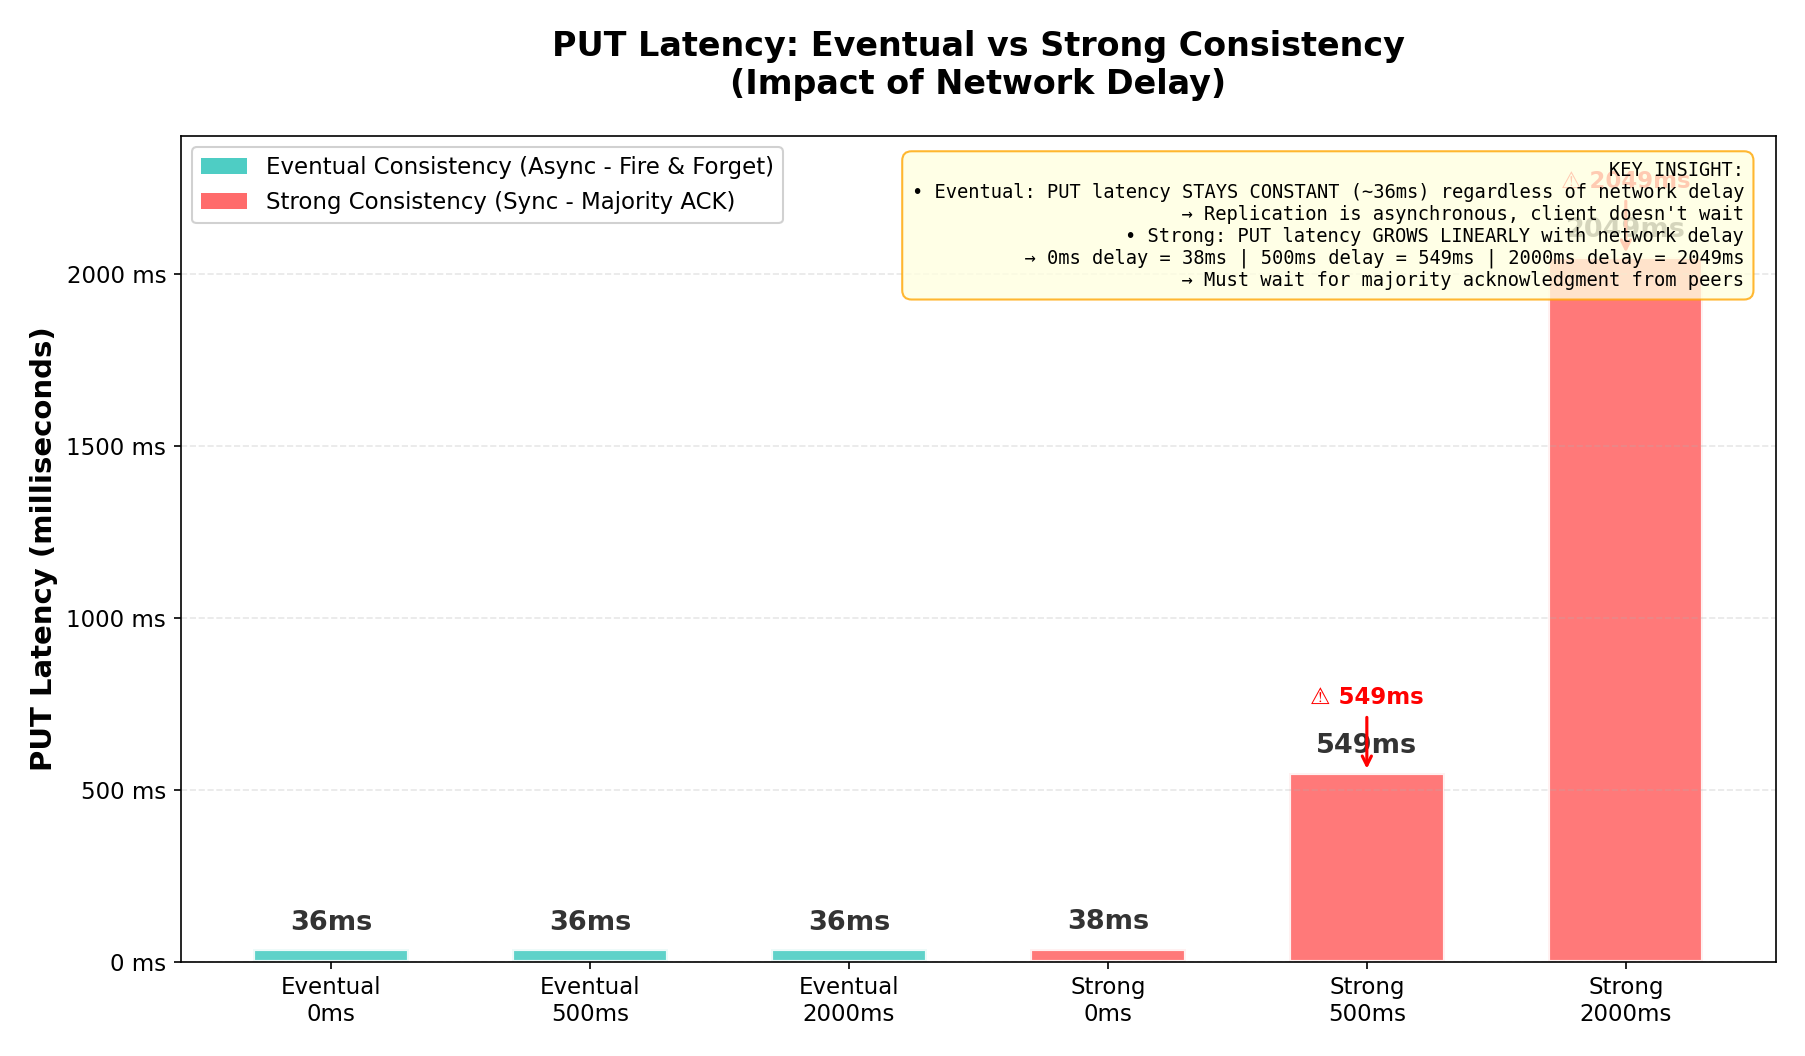
\includegraphics[width=0.82\textwidth]{../report/charts/01_PUT_Latency_Comparison.png}
\caption{مقایسه تاخیر عملیات PUT بین مدل Eventual و Strong}
\end{figure}

\begin{figure}[H]
\centering
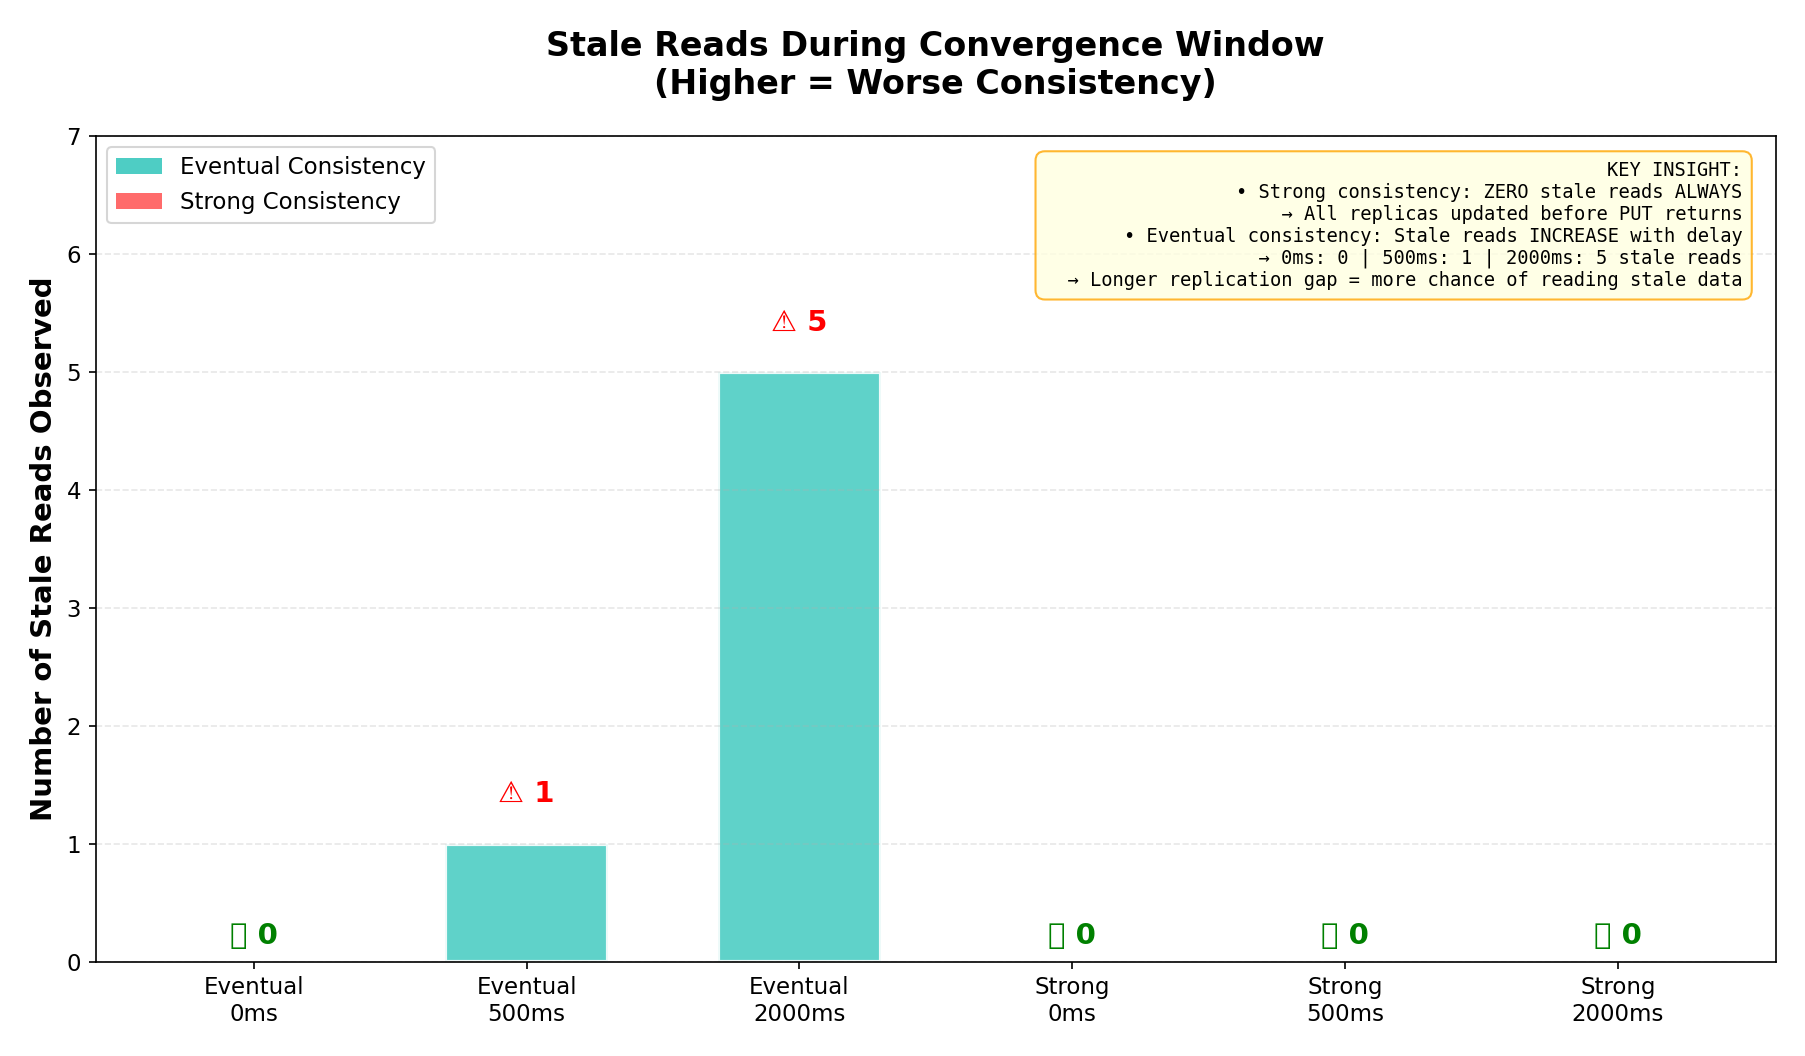
\includegraphics[width=0.82\textwidth]{../report/charts/02_Stale_Reads_Comparison.png}
\caption{تعداد خواندن‌های کهنه (Stale Reads) در سناریوهای مختلف تاخیر شبکه}
\end{figure}

\begin{figure}[H]
\centering
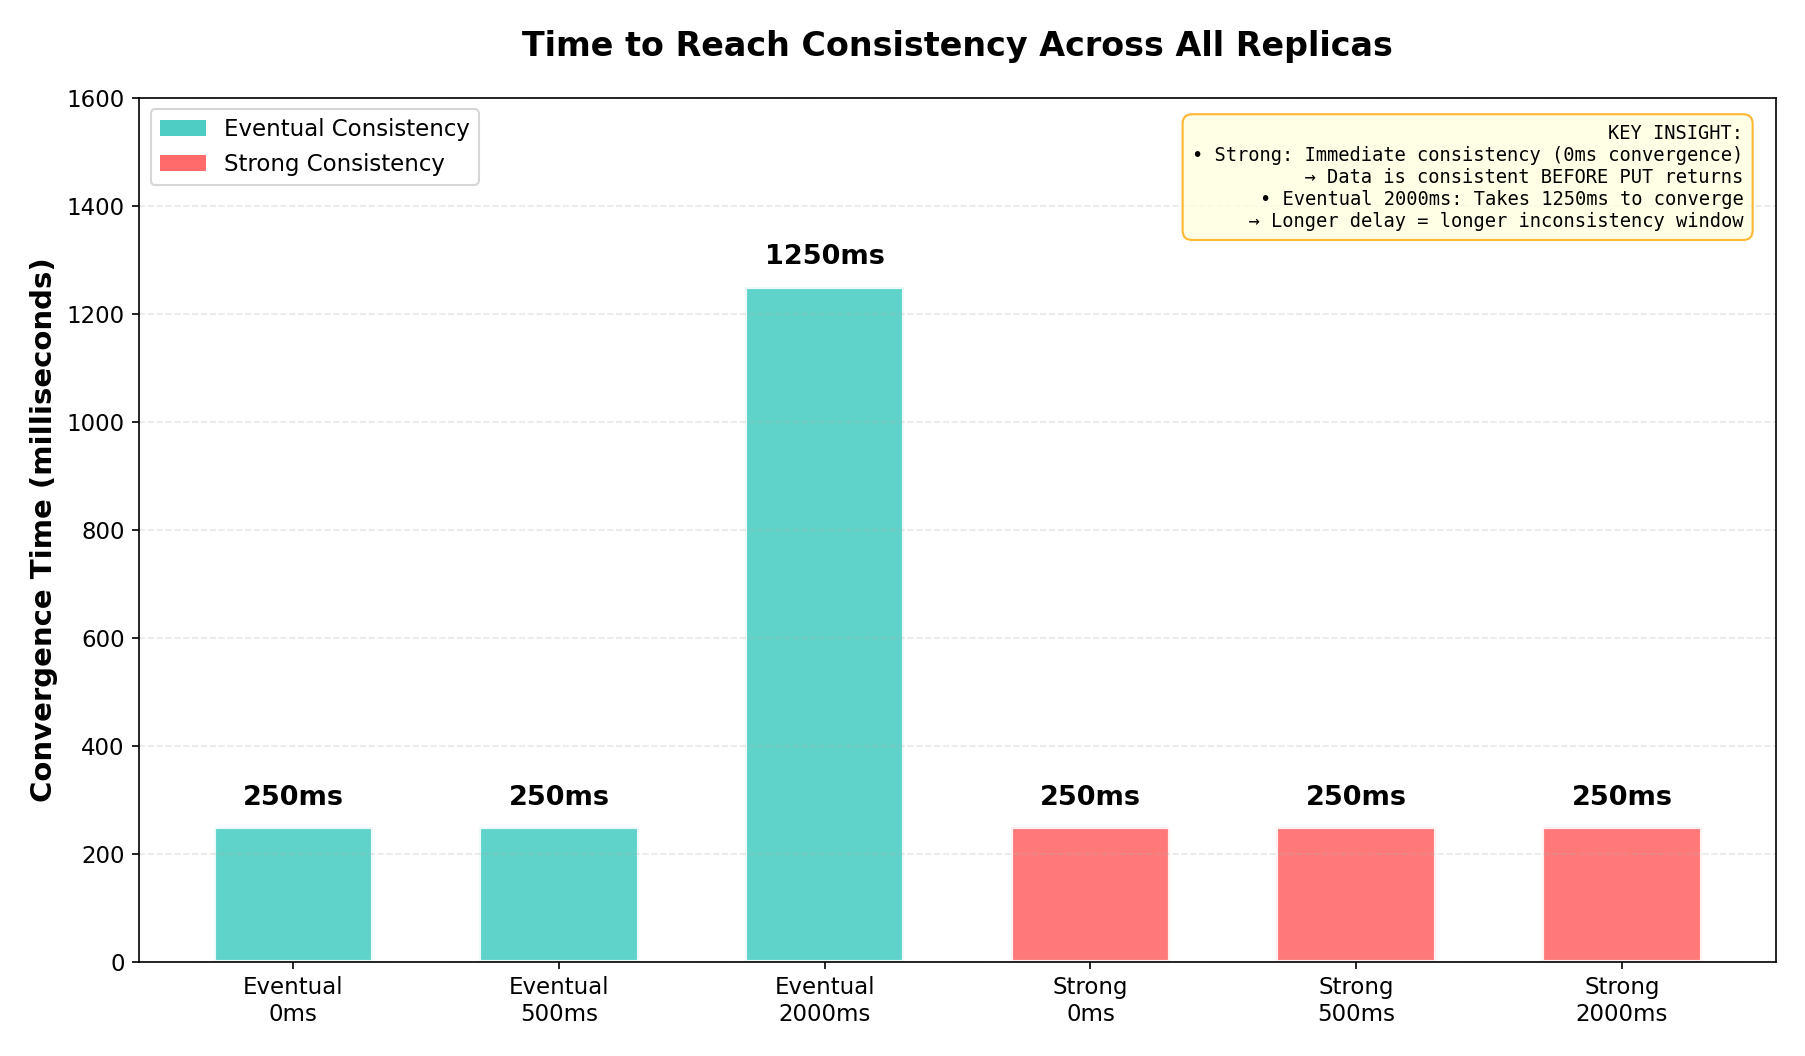
\includegraphics[width=0.82\textwidth]{../report/charts/03_Convergence_Time.png}
\caption{زمان همگرایی نودها (Convergence Time) در تاخیرهای شبکه}
\end{figure}

\begin{figure}[H]
\centering
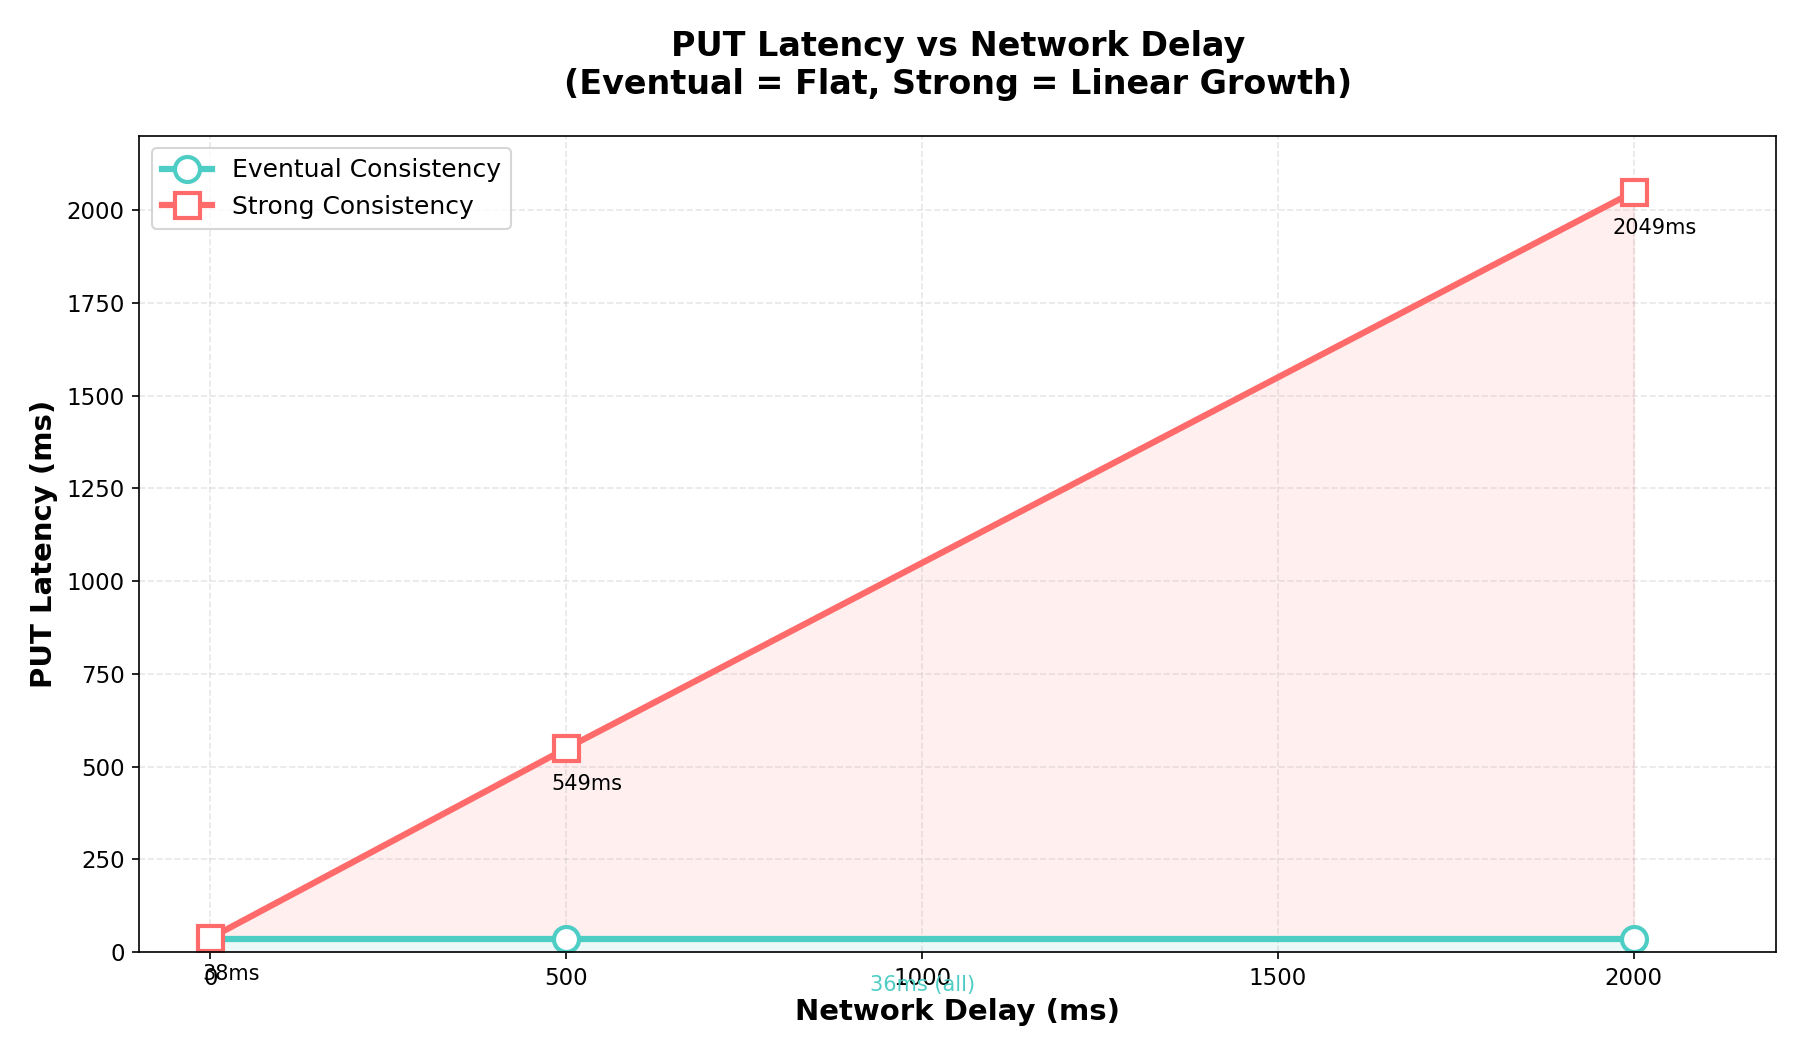
\includegraphics[width=0.82\textwidth]{../report/charts/04_PUT_Latency_vs_Delay.png}
\caption{روند تغییرات تاخیر PUT متناسب با افزایش تاخیر شبکه}
\end{figure}

\begin{figure}[H]
\centering
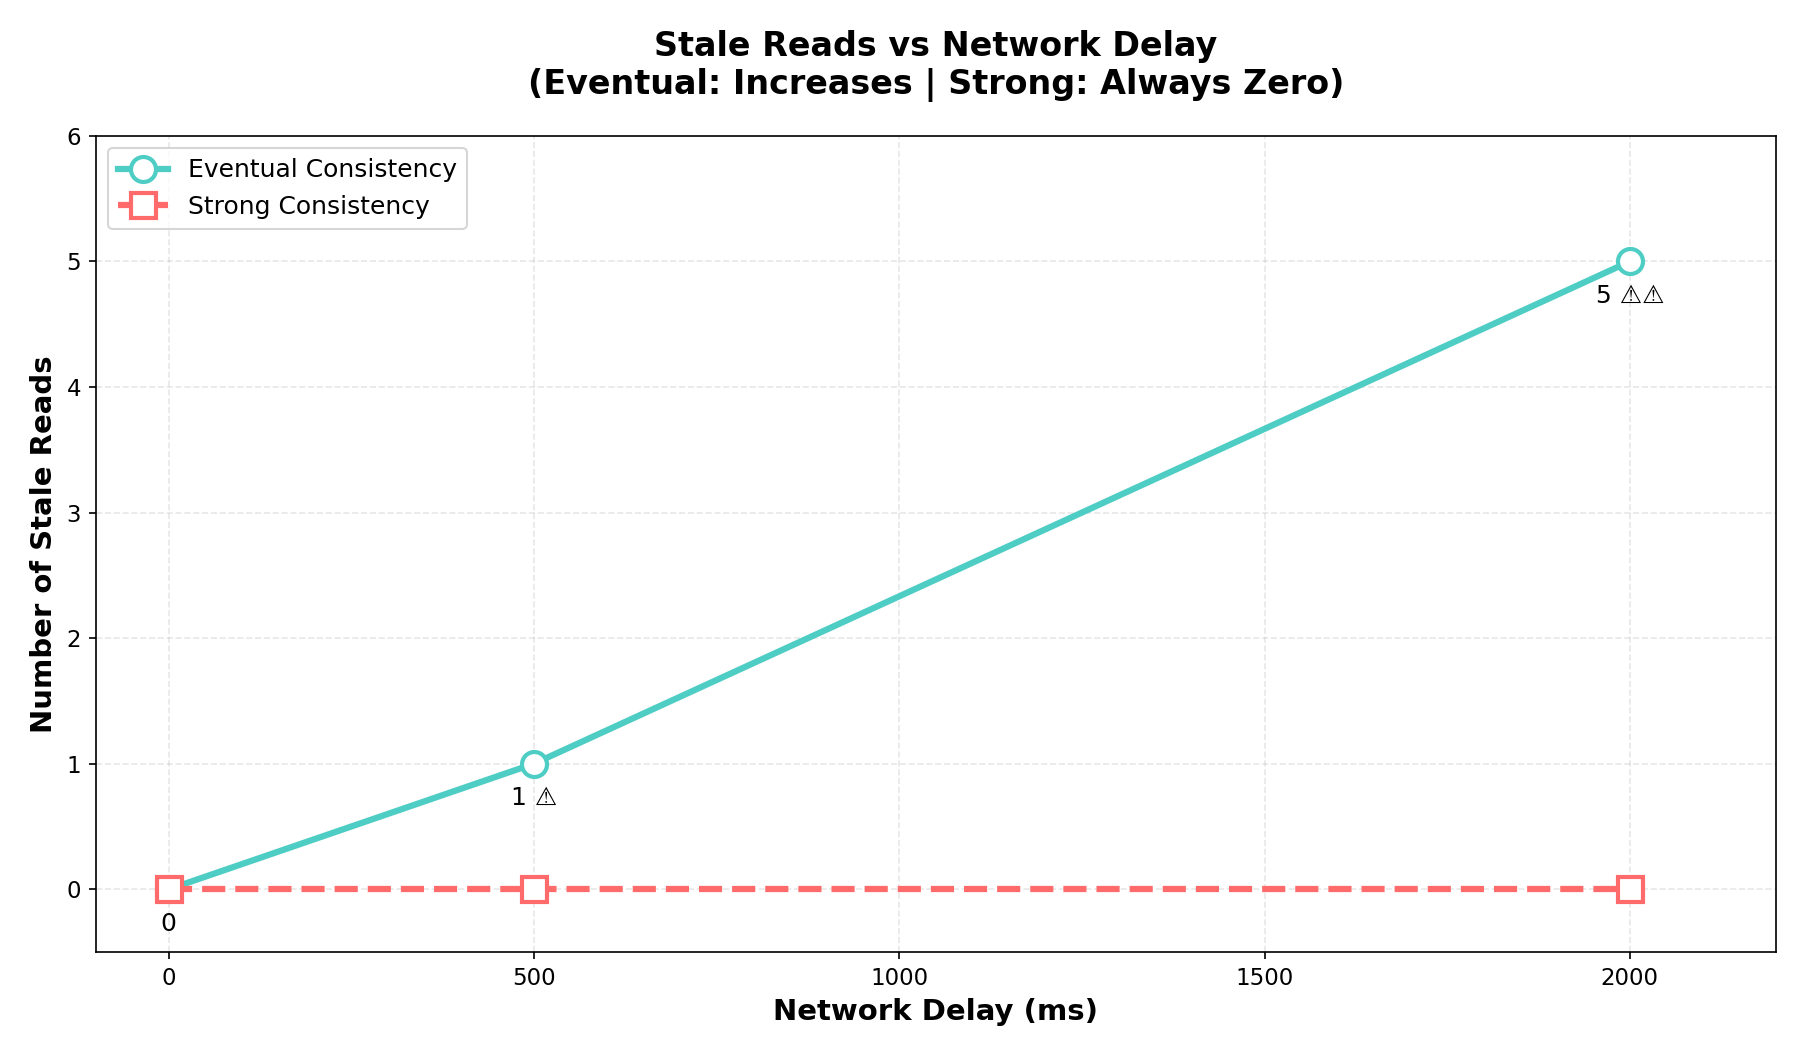
\includegraphics[width=0.82\textwidth]{../report/charts/05_Stale_Reads_vs_Delay.png}
\caption{تاثیر تاخیر شبکه بر افزایش تعداد Stale Reads در مدل Eventual}
\end{figure}

\begin{figure}[H]
\centering
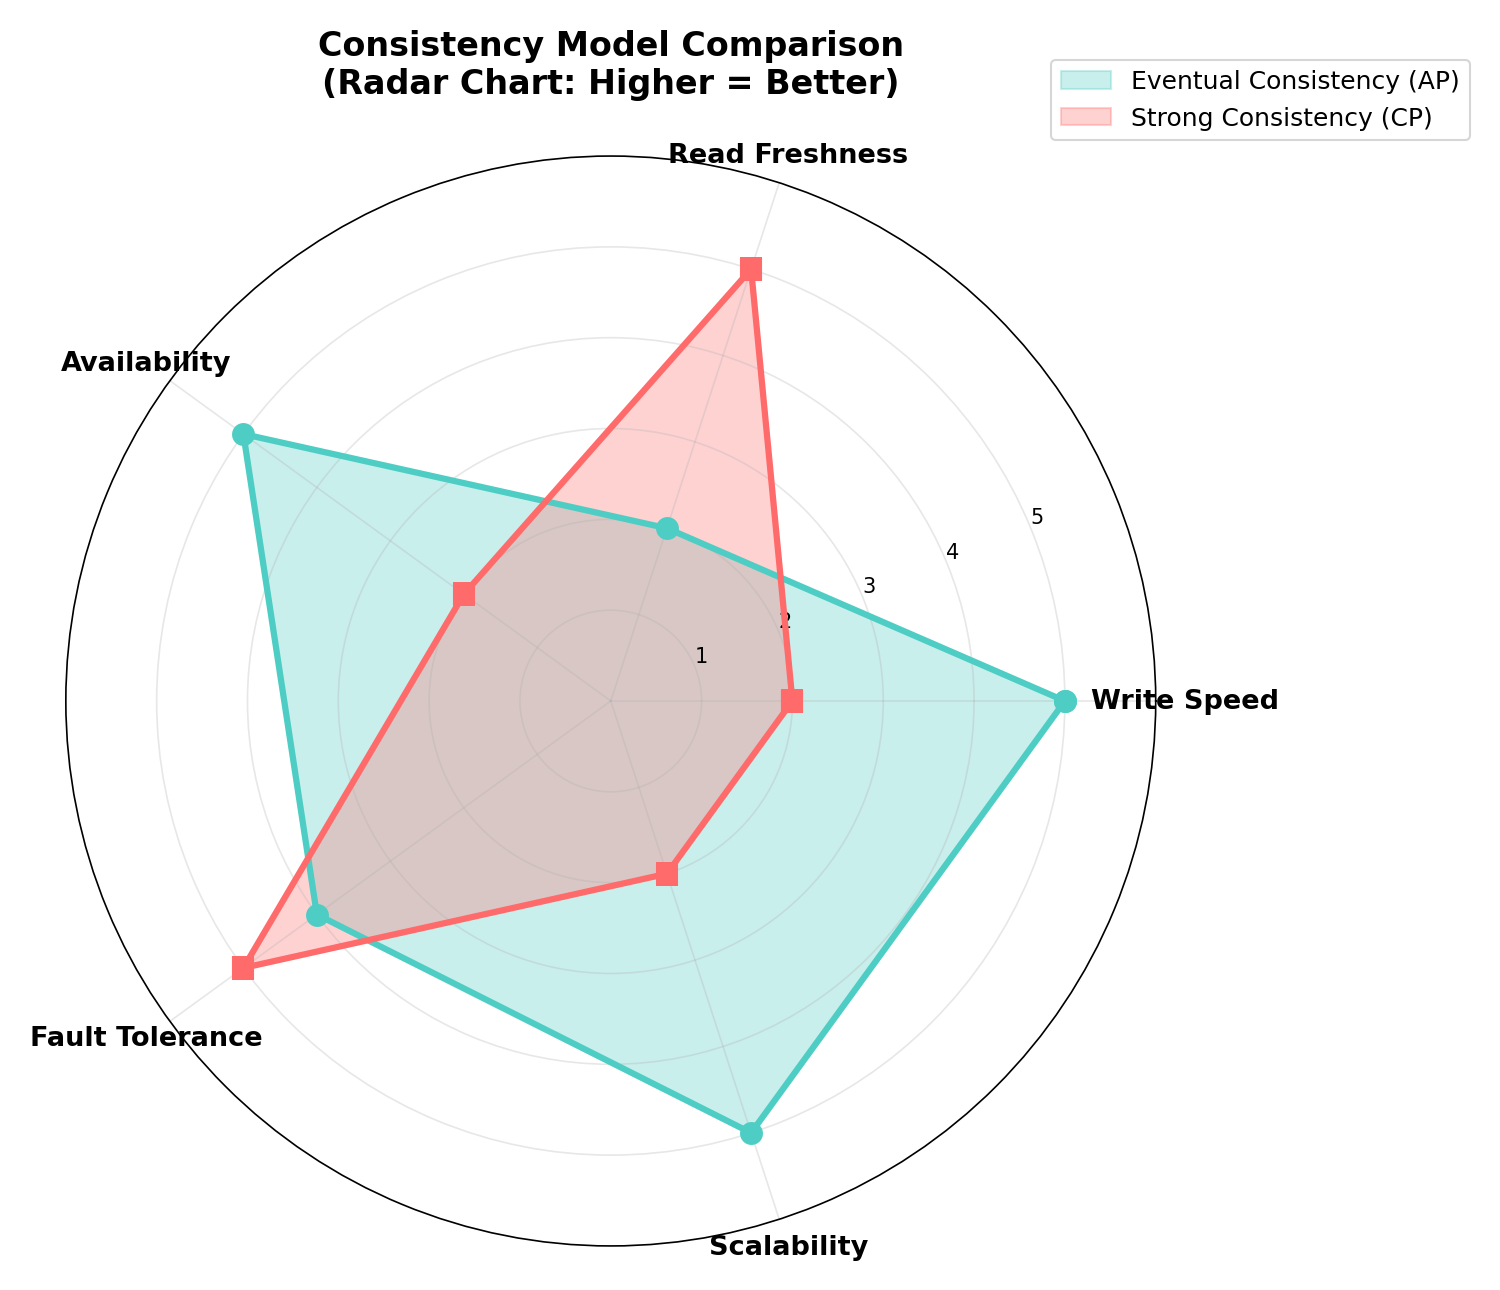
\includegraphics[width=0.82\textwidth]{../report/charts/06_Radar_Chart_Comparison.png}
\caption{نمودار راداری مقایسه سناریوهای مختلف سیستم طبق قضیه CAP}
\end{figure}

\begin{figure}[H]
\centering
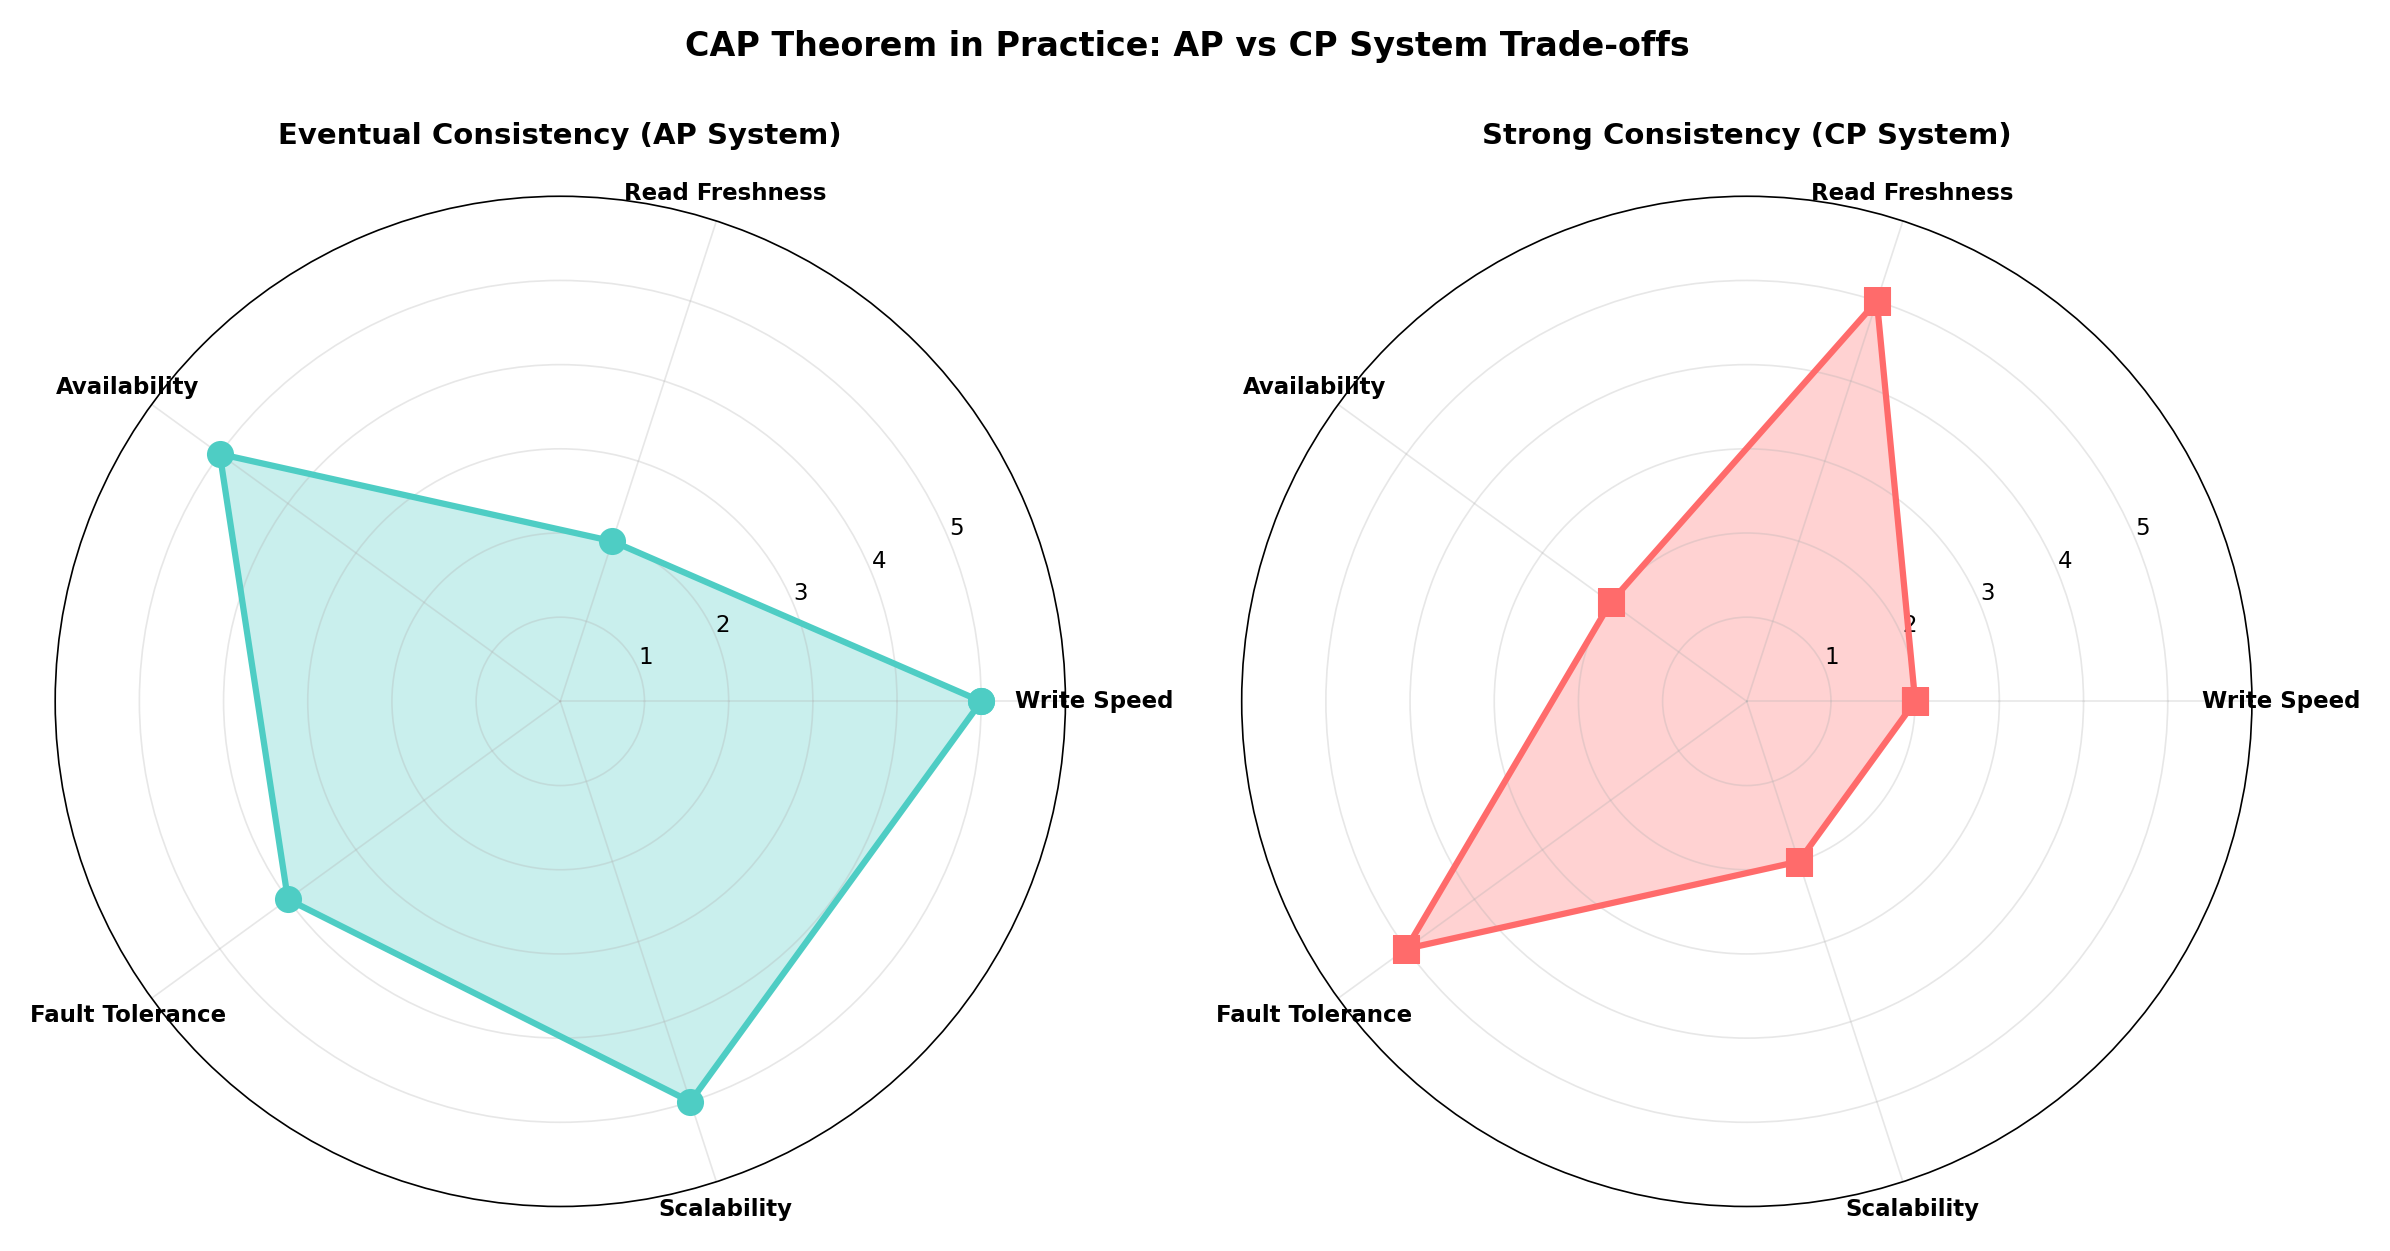
\includegraphics[width=0.82\textwidth]{../report/charts/07_Dual_Radar_Charts.png}
\caption{مقایسه راداری دوگانه Eventual Consistency در برابر Strong Quorum}
\end{figure}

\begin{figure}[H]
\centering
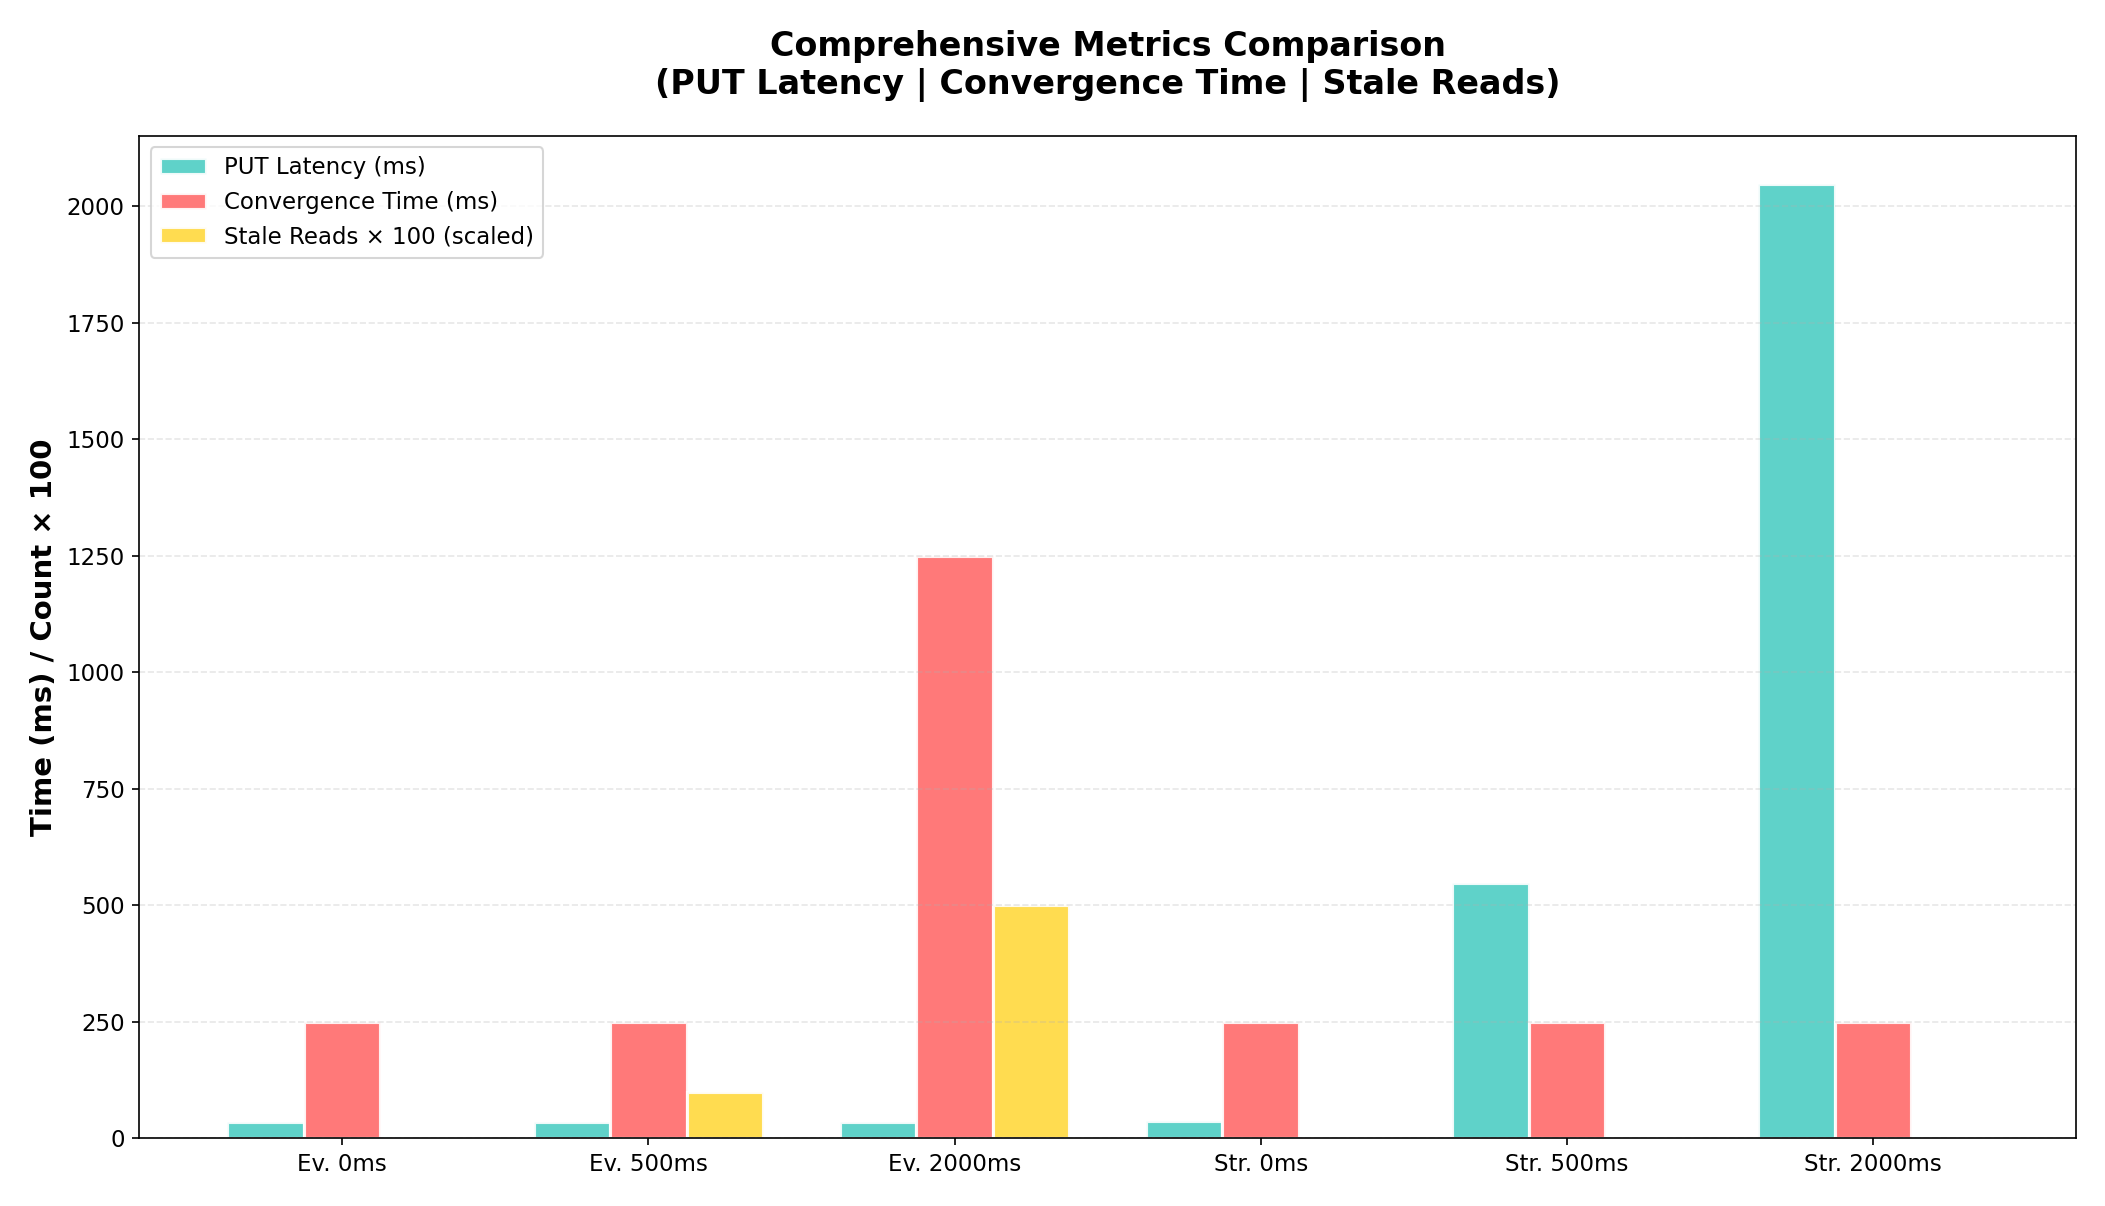
\includegraphics[width=0.82\textwidth]{../report/charts/08_Grouped_Bar_All_Metrics.png}
\caption{نمودار میله‌ای مجتمع کلیه متریک‌های کلیدی سیستم}
\end{figure}

\begin{figure}[H]
\centering
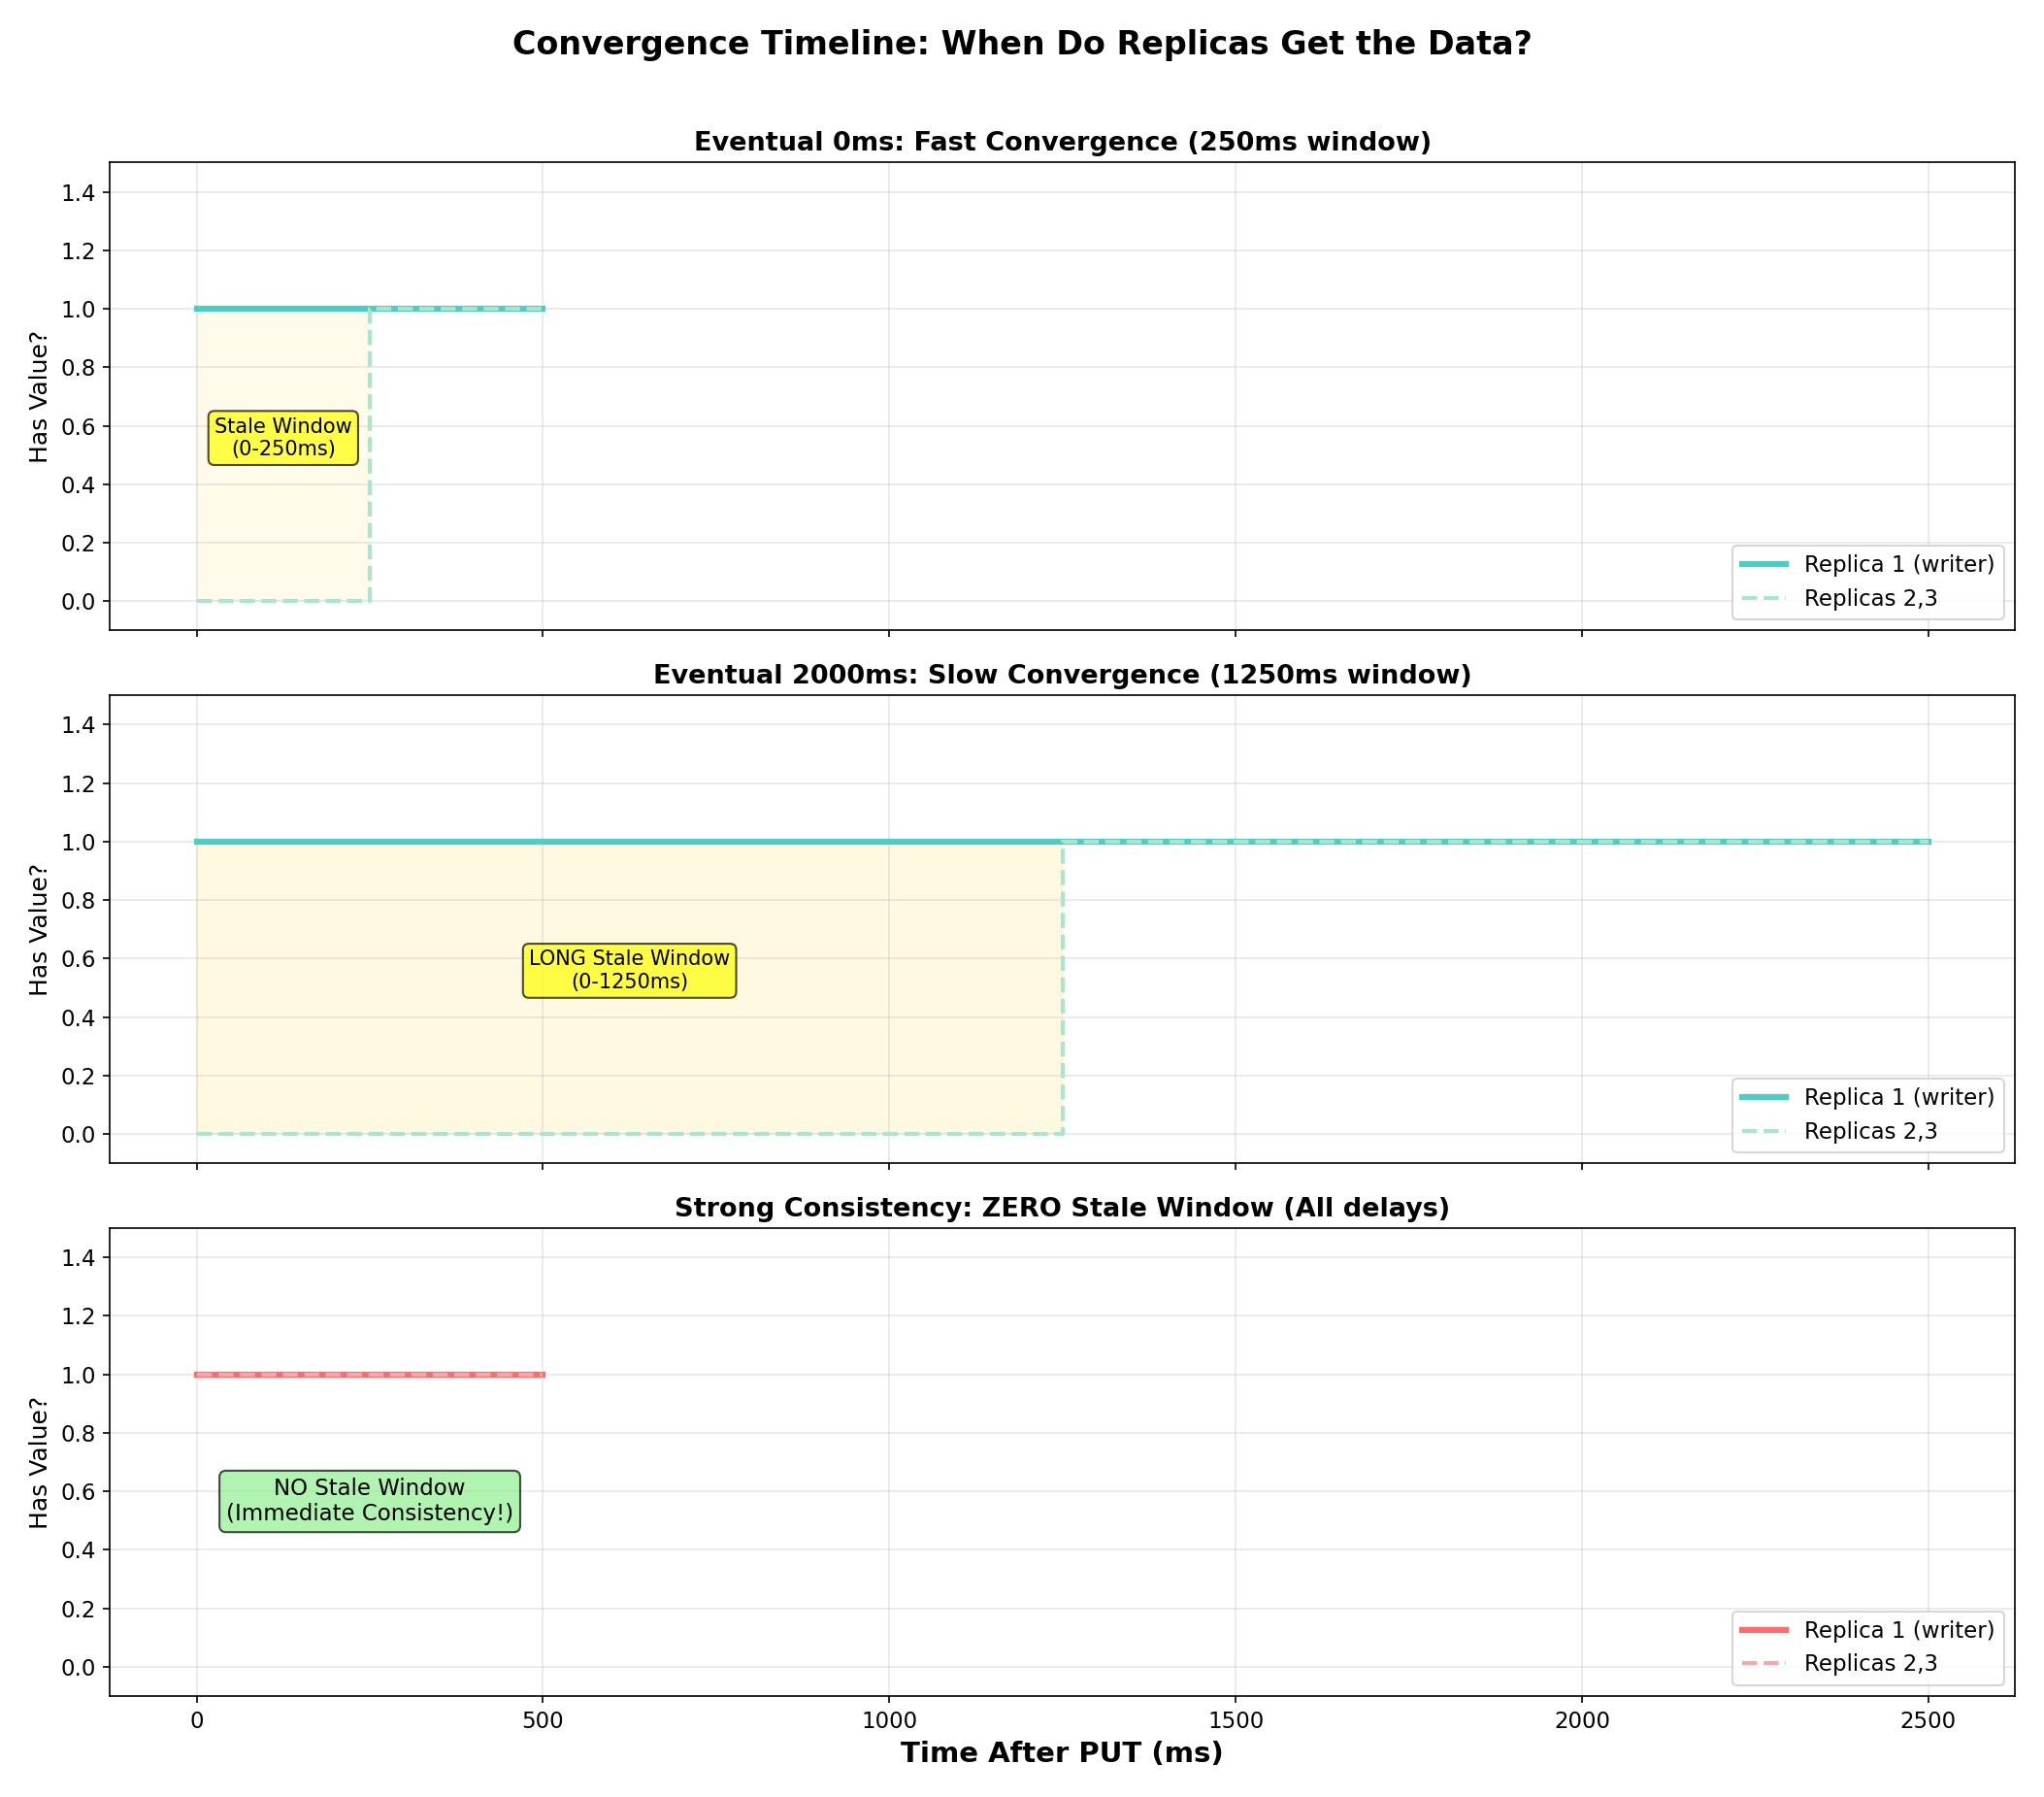
\includegraphics[width=0.92\textwidth]{../report/charts/09_Convergence_Timeline.png}
\caption{خط زمانی همگرایی نودها و انتشار به‌روزرسانی‌ها}
\end{figure}

\begin{figure}[H]
\centering
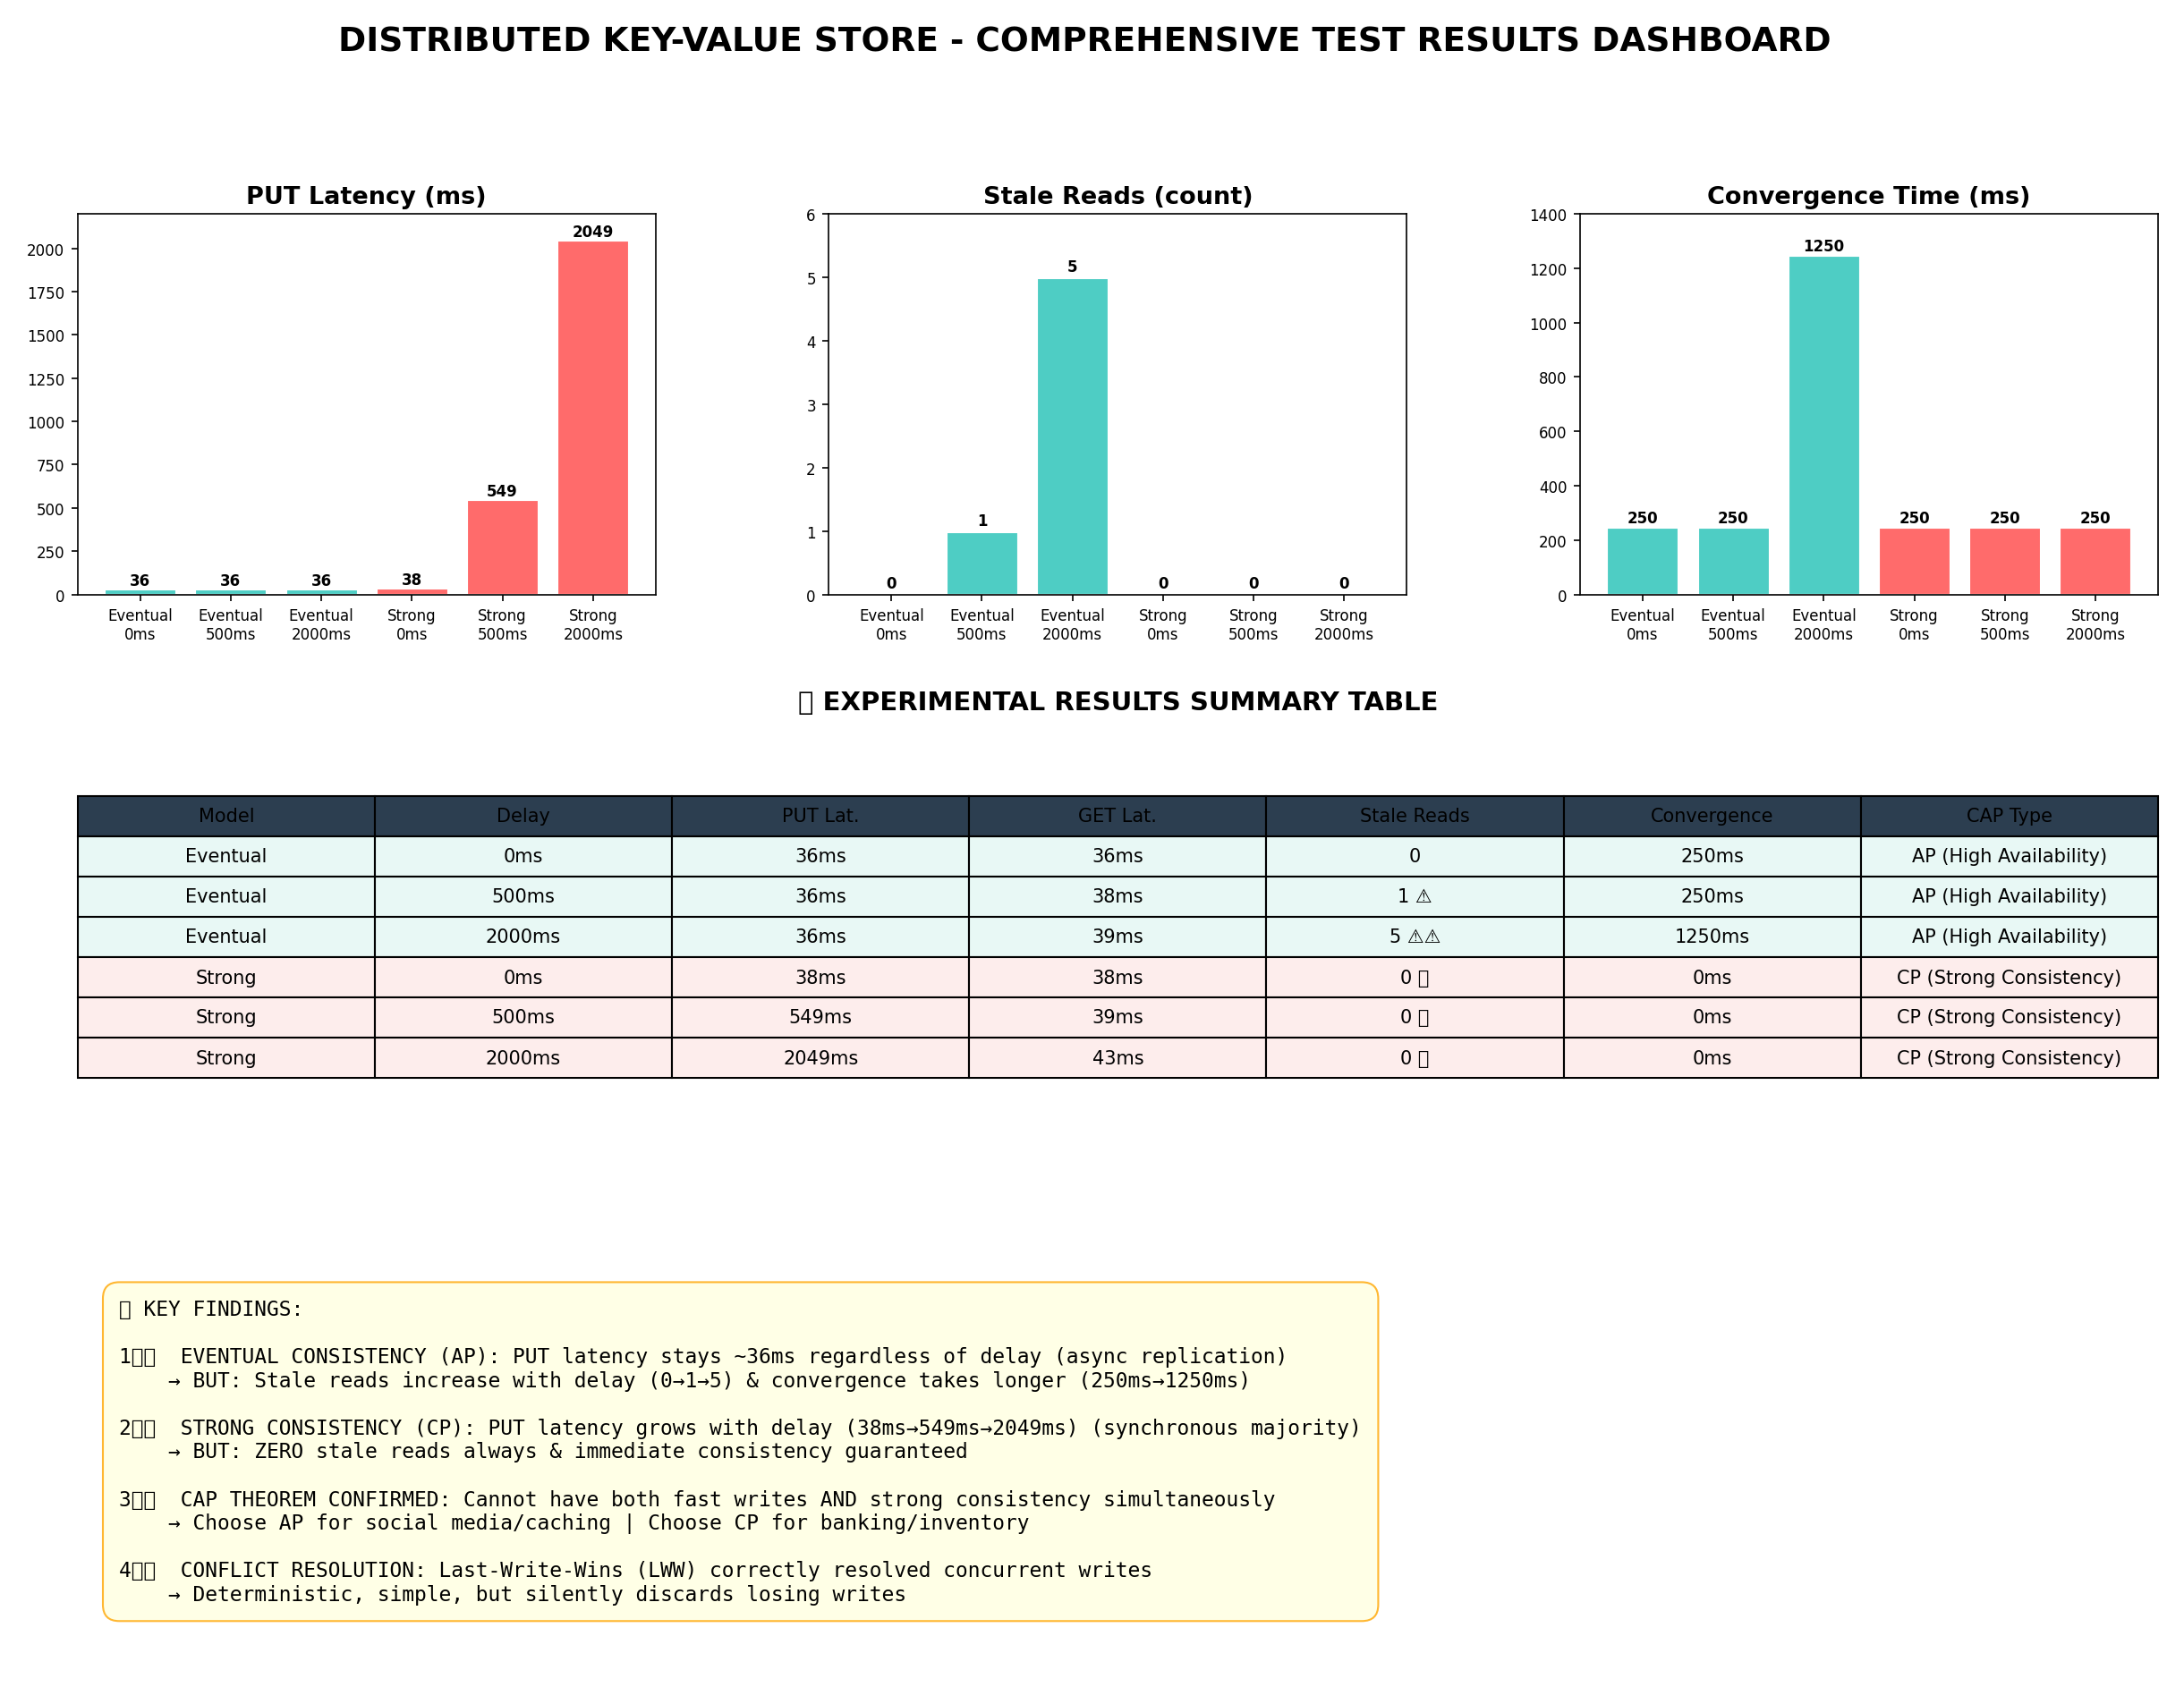
\includegraphics[width=0.95\textwidth]{../report/charts/10_Summary_Dashboard.png}
\caption{داشبورد خلاصه مدیریتی ارزیابی کارایی پایگاه داده توزیع‌شده}
\end{figure}

% ----------------------------------------------------------------------------
% ۵. راهنمای دفاع و نتیجه‌گیری
% ----------------------------------------------------------------------------
\section{نتیجه‌گیری و راهنمای جلسه دفاع}

\subsection{نتیجه‌گیری}
ارزیابی تجربی سیستم تایید کرد که:
\begin{enumerate}
    \item در مدل \textbf{Eventual Consistency (AP)}، تاخیر PUT بسیار پایین و مستقل از تاخیر شبکه است، اما با افزایش تاخیر شبکه احتمال Stale Read افزایش می‌یابد.
    \item در مدل \textbf{Strong Consistency (CP)}، هیچ خواندن کهنه‌ای رخ نمی‌دهد، اما تاخیر عملیات نوشتن متناسب با تاخیر شبکه تا بیش از ۲ ثانیه افزایش می‌یابد.
\end{enumerate}

\subsection{راهنمای دفاع (Q\&A Defense Guide)}
\begin{itemize}
    \item \textbf{سوال: در مدل Strong اگر یک نود خرابی کند چه می‌شود؟}\\
    \textbf{پاسخ:} حد نصاب اکثریت برای ۳ نود برابر ۲ نود است ($3/2 + 1 = 2$). تا زمانی که ۲ نود سالم باشند، سیستم به نوشتن ادامه می‌دهد. اگر ۲ نود خاموش شوند، جهت حفظ سازگاری درخواست نوشتن رد می‌شود.
    \item \textbf{سوال: چالش اصلی الگوریتم LWW چیست؟}\\
    \textbf{پاسخ:} انحراف ساعت سرورها (Clock Skew). برای رفع این چالش در سیستم‌های واقعی مانند Cassandra یا Spanner از Vector Clocks یا TrueTime API استفاده می‌شود.
\end{itemize}

\end{document}
